%% ============================================================
%%  SECCIÓN 5 — Materiales y Equipos
%% ============================================================

\section{Materiales y Equipos}
\label{sec:materiales}

A continuación se detallan los instrumentos de medición, fuentes de excitación y elementos circuitales empleados durante la sesión experimental, con sus especificaciones técnicas y metrológicas.

\subsection{Fuente de Alimentación de Corriente Continua (DC)}
\begin{itemize}
    \item \textbf{Descripción y función:} Fuente de tensión continua regulada de laboratorio, empleada como generador de potencial primario constante para alimentar el circuito divisor resistivo. Se configuró en una salida nominal de \qty{7,5}{\volt} DC.
    \item \textbf{Especificaciones técnicas:} Rango de salida \qtyrange{0}{30}{\volt}, rizado de salida $< \qty{1}{\milli\voltrms}$, estabilidad de línea $\pm\qty{0,01}{\percent}$.
    \item \textbf{Incertidumbre instrumental:} $\delta V_s = \pm(\qty{0,5}{\percent} + \qty{0,05}{\volt})$.
    \item \textbf{Precauciones operativas:} Verificación de polaridad antes de energizar la red y control de no cortocircuitar los bornes de salida.
\end{itemize}

\begin{figure}[H]
    \centering
    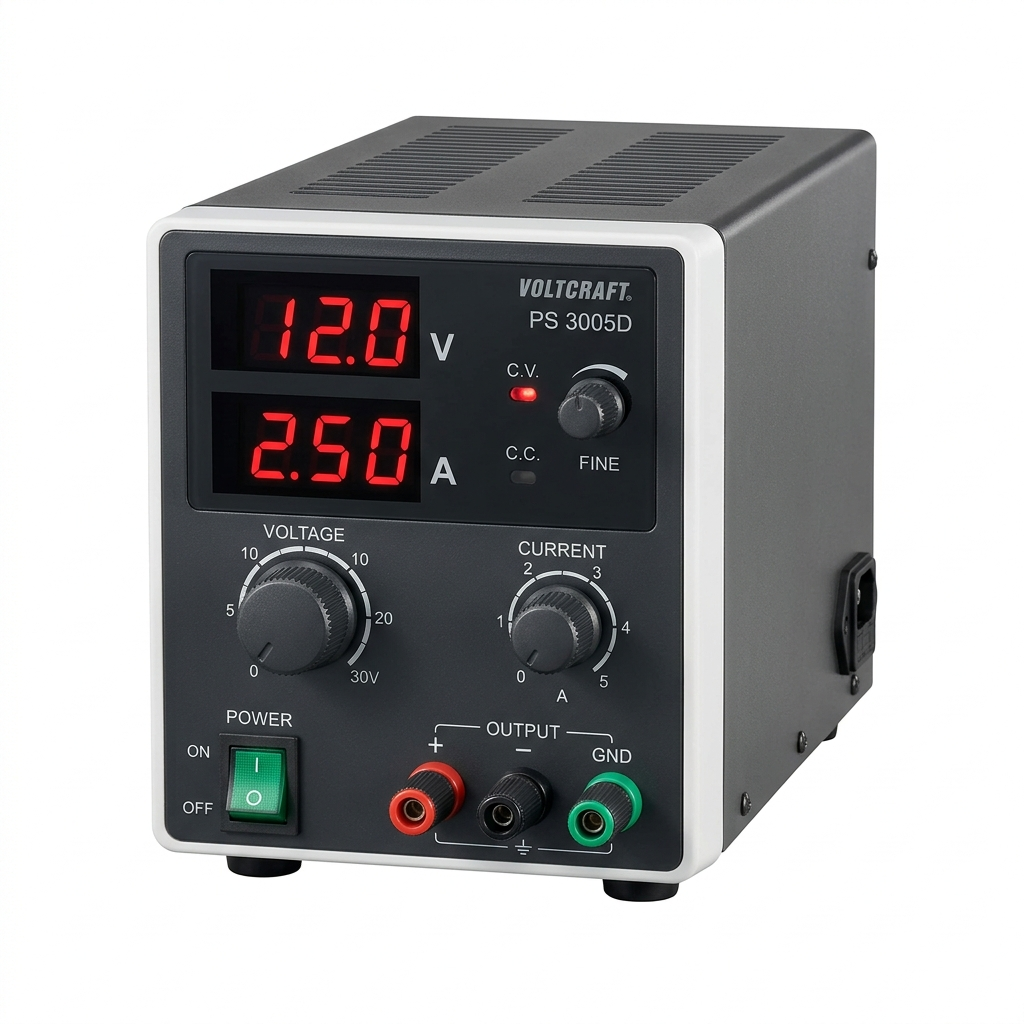
\includegraphics[width=0.50\linewidth, height=5.5cm]{fig_fuente_dc}
    \caption{Fuente de alimentación regulada de corriente continua empleada en el laboratorio.}
    \label{fig:mat_fuente_dc}
\end{figure}

\subsection{Medidor Digital Multifunción (Voltímetro y Amperímetro Digital)}
\begin{itemize}
    \item \textbf{Descripción y función:} Instrumento digital de alta precisión para la adquisición simultánea de la diferencia de potencial $V$ en bornes del componente y la intensidad de corriente $I$ que circula a través del mismo.
    \item \textbf{Especificaciones técnicas:}
    \begin{itemize}
        \item Escala de voltímetro DC: rango \qtyrange{0,00}{20,00}{\volt}, resolución de display $\qty{0,01}{\volt}$, impedancia de entrada $R_{\text{in}} \ge \qty{10}{\mega\ohm}$. Tolerancia de fabricante: $\pm(\qty{0,5}{\percent}\,\text{lectura} + 2\text{ dígitos})$.
        \item Escala de amperímetro DC: rango \qtyrange{0,000}{2,000}{\ampere}, resolución de display $\qty{0,001}{\ampere}$, caída de potencial de inserción mínima (baja resistencia shunt interna). Tolerancia de fabricante: $\pm(\qty{1,0}{\percent}\,\text{lectura} + 3\text{ dígitos})$.
    \end{itemize}
    \item \textbf{Incertidumbres Tipo B de lectura:} En las escalas operativas utilizadas, las resoluciones instrumentales dominantes son $\delta V = \pm\qty{0,01}{\volt}$ y $\delta I = \pm\qty{0,001}{\ampere}$.
    \item \textbf{Precauciones operativas:} Inserción estricta del amperímetro en serie con la carga para evitar sobrecorrientes destructivas y conexión del voltímetro en paralelo directo entre los nodos $a$ y $b$.
\end{itemize}

\begin{figure}[H]
    \centering
    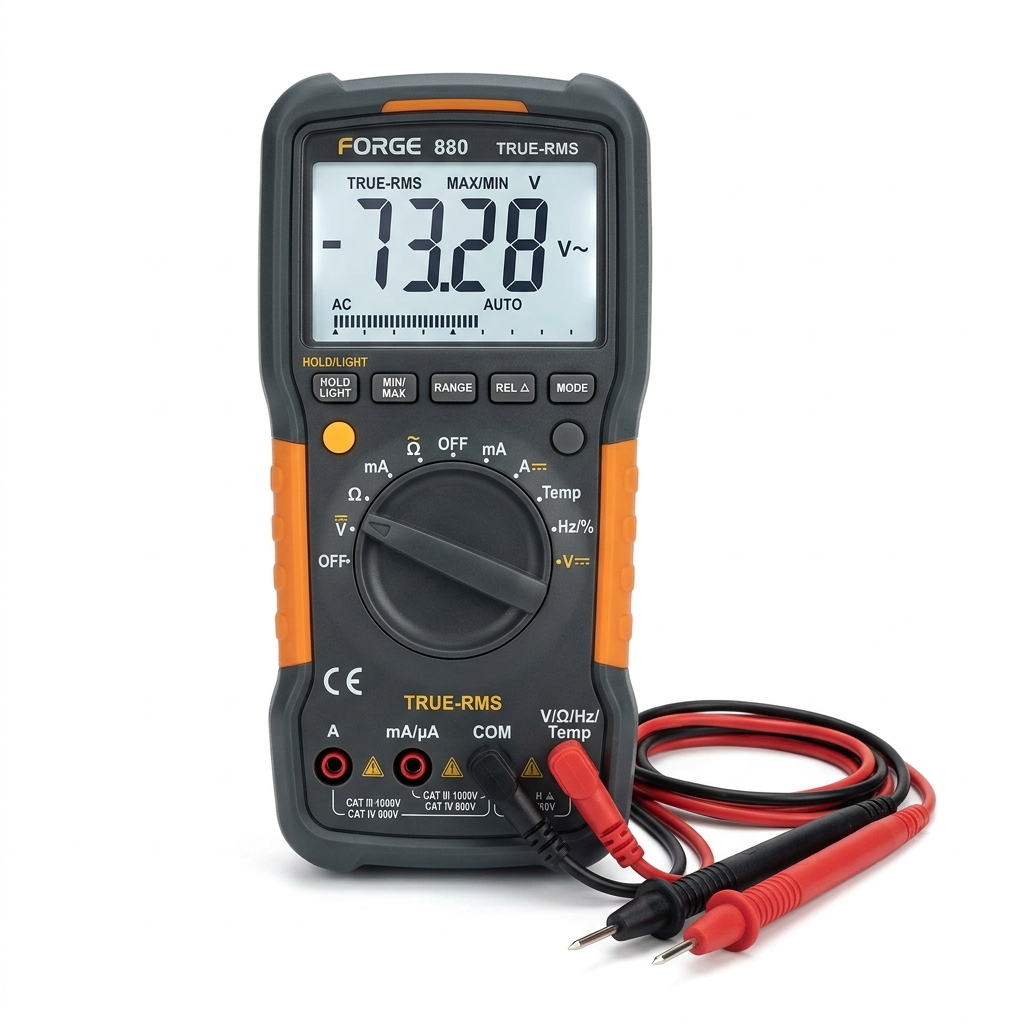
\includegraphics[width=0.50\linewidth, height=5.5cm]{fig_multimetro}
    \caption{Medidor digital de precisión empleado para el registro simultáneo de potencial y corriente.}
    \label{fig:mat_multimetro}
\end{figure}

\subsection{Reóstato de Laboratorio (Potenciómetro Divisor de Tensión)}
\begin{itemize}
    \item \textbf{Descripción y función:} Dispositivo resistivo de hilo arrollado sobre núcleo cerámico provisto de un cursor deslizante metálico. Se conectó en configuración de tres terminales (potenciómetro) para operar como un divisor de voltaje de relación continua $x \in [0, 1]$.
    \item \textbf{Especificaciones técnicas:} Resistencia nominal total $R_p \approx \qty{330}{\ohm}$, corriente máxima admisible \qty{1,5}{\ampere}.
    \item \textbf{Precauciones operativas:} Desplazamiento suave del cursor para no dañar las espiras del bobinado y verificación de disipación térmica cuando el cursor se sitúa cerca del extremo superior.
\end{itemize}

\begin{figure}[H]
    \centering
    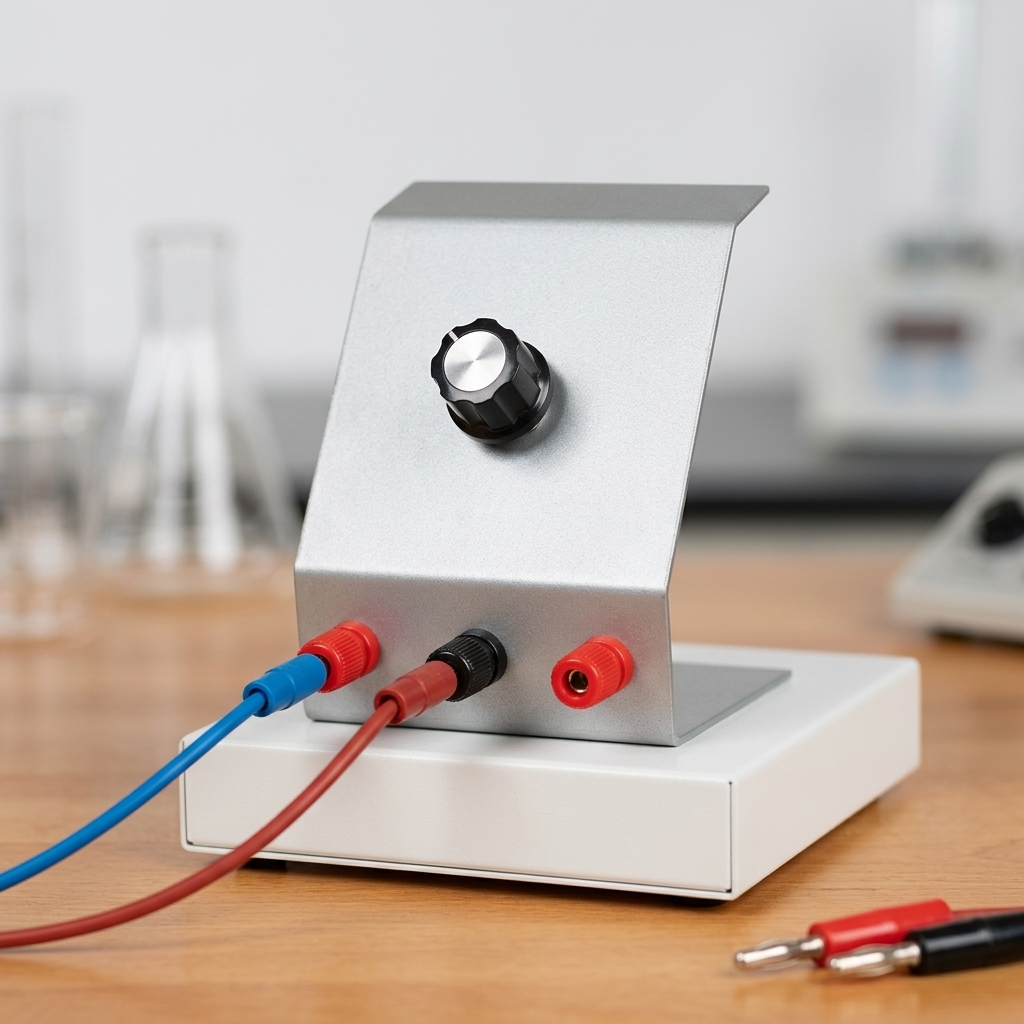
\includegraphics[width=0.50\linewidth, height=5.5cm]{fig_reostato}
    \caption{Unidad potencimétrica de laboratorio provista de cursor rotativo y bornes de derivación.}
    \label{fig:mat_reostato}
\end{figure}

\subsection{Caja de Elementos de Prueba y Cargas Resistivas}
La caja de prueba de laboratorio contiene los componentes bajo análisis:
\begin{enumerate}
    \item \textbf{Elemento E1 --- Lámpara incandescente:} Foco miniatura con ampolla de vidrio al vacío y filamento de tungsteno bobinado, tensión nominal \qty{6}{\volt}, corriente máxima de régimen continuo \qty{0,5}{\ampere}, resistencia en caliente de diseño $\approx \qtyrange{12}{15}{\ohm}$.
    \item \textbf{Elemento E2 --- Resistencia de composición de carbón:} Resistor cerámico comercial de valor nominal $R_{\text{nom}} = \qty{100}{\ohm}$ con tolerancia de fabricante de $\pm\qty{5}{\percent}$ (código de bandas: marrón-negro-marrón-oro~\cite{vishay_resistors}), potencia máxima de disipación de \qty{1}{\watt}.
    \item \textbf{Elemento E3 --- Diodo semiconductor de silicio:} Diodo rectificador de juntura $p$-$n$ de silicio estándar (serie 1N4007, encapsulado DO-41~\cite{vishay_1n4007}), corriente directa media máxima $I_{\text{F,max}} = \qty{1,0}{\ampere}$, caída de tensión directa típica $V_F \approx \qtyrange{0,7}{1,1}{\volt}$, tensión inversa de pico repetitivo $V_{\text{RRM}} = \qty{1000}{\volt}$ y resistencia térmica unión-ambiente $R_{\theta JA} = \qty{50}{\celsius\per\watt}$. Límite operativo fijado en el laboratorio para evitar degradación térmica: $I \le \qty{0,900}{\ampere}$.
\end{enumerate}

\begin{figure}[H]
    \centering
    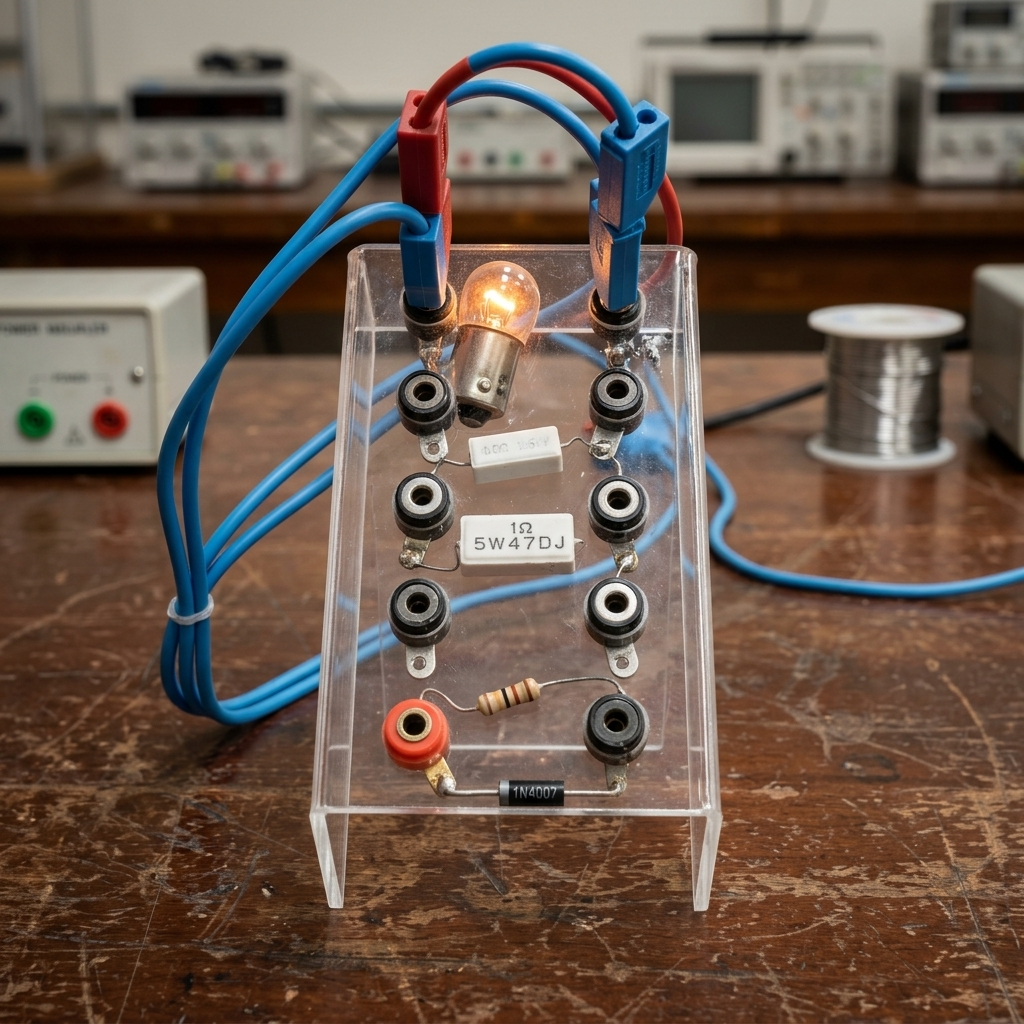
\includegraphics[width=0.50\linewidth, height=5.5cm]{fig_caja_elementos}
    \caption{Módulo acrílico de prueba del laboratorio con los dipolos ensayados: lámpara incandescente de tungsteno en emisión (E1), resistencias de potencia y carbón de \qty{100}{\ohm} (E2), y diodo rectificador de silicio (E3).}
    \label{fig:mat_caja_elementos}
\end{figure}

\subsection{Cables de Conexión y Terminales Banana--Caimán}
\begin{itemize}
    \item \textbf{Descripción y función:} Ocho conductores de cobre multifilar flexible con aislamiento termoplástico de seguridad, equipados con conectores tipo banana apilables de \qty{4}{\milli\meter} y conectores tipo caimán protegidos para el acoplamiento a los bornes de la caja de elementos.
    \item \textbf{Resistencia de contacto parásita:} $R_{\text{cable}} \le \qty{0,03}{\ohm}$ por línea, despreciable frente a las impedancias de los elementos ensayados.
\end{itemize}

\begin{figure}[H]
    \centering
    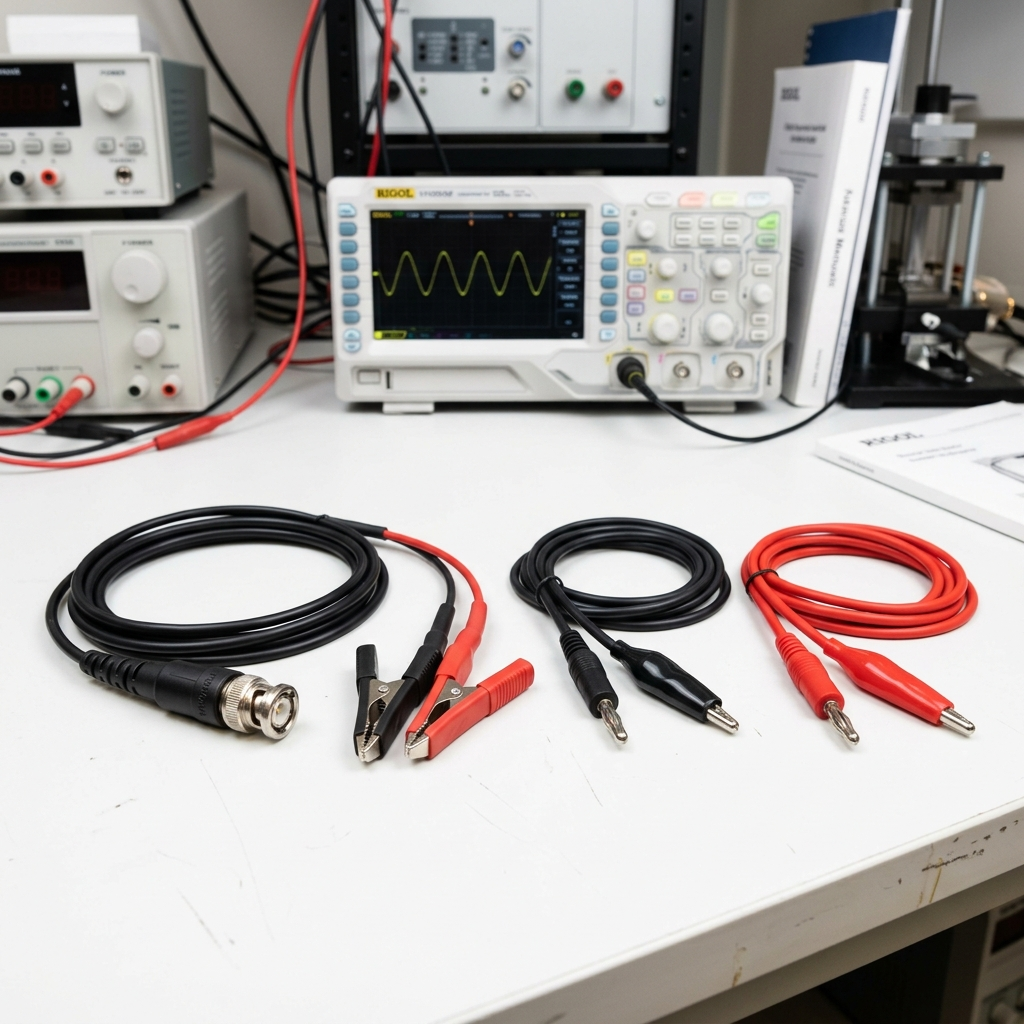
\includegraphics[width=0.50\linewidth, height=5.5cm]{fig_cables_sondas}
    \caption{Juego de cables conductores y sondas de laboratorio con conectores banana y caimán.}
    \label{fig:mat_cables}
\end{figure}

\subsection{Tabla Metrológica Resumen de Instrumentación}
En la Tabla~\ref{tab:especificaciones_equipos} se sintetiza el cuadro metrológico completo de los instrumentos utilizados, detallando sus intervalos de trabajo, apreciaciones mínimas y tolerancias analíticas.

\begin{table}[H]
    \centering
    \caption{Especificaciones metrológicas de los equipos e instrumentos de laboratorio empleados.}
    \label{tab:especificaciones_equipos}
    \resizebox{\linewidth}{!}{%
    \begin{tabular}{@{}lllcc@{}}
        \toprule
        \textbf{Instrumento / Equipo} & \textbf{Marca / Modelo} & \textbf{Rango de Operación} & \textbf{Resolución} & \textbf{Incertidumbre Combinada} \\
        \midrule
        Fuente DC de Laboratorio      & Regulada Dual           & \qtyrange{0}{30}{\volt}     & \qty{0,05}{\volt}   & $\pm(\qty{0,5}{\percent} + \qty{0,05}{\volt})$ \\
        Voltímetro Digital            & Medidor Automático DC   & \qtyrange{0}{20}{\volt}     & \qty{0,01}{\volt}   & $\pm(\qty{0,2}{\percent} + \qty{0,01}{\volt})$ \\
        Amperímetro Digital           & Medidor Automático DC   & \qtyrange{0}{2}{\ampere}    & \qty{0,001}{\ampere}& $\pm(\qty{0,3}{\percent} + \qty{0,001}{\ampere})$ \\
        Reóstato de Laboratorio       & Tipo Potenciómetro      & \qtyrange{0}{330}{\ohm}     & Continua            & $\pm\qty{5}{\percent}$ nominal \\
        Resistor Patrón (E2)          & Carbón Prensado         & Nominal \qty{100}{\ohm}     & —                   & Tolerancia $\pm\qty{5}{\percent}$ (\qty{5}{\ohm}) \\
        Diodo Silicio (E3)            & Unión $p$-$n$ 1N400x    & $I \le \qty{0,9}{\ampere}$  & —                   & $V_u \approx \qtyrange{0,6}{0,7}{\volt}$ \\
        Lámpara de Tungsteno (E1)     & Filamento Miniatura     & \qtyrange{0}{6,5}{\volt}    & —                   & $P_{\text{max}} \approx \qty{3}{\watt}$ \\
        \bottomrule
    \end{tabular}%
    }
\end{table}